\begin{dfn}[Ordered Geometry]
Let \(P\) be an incidence geometry with a betweenness relation \(\BETWEEN{\ast}{\ast}{\ast}\).
We say that \(P\) is an \emph{ordered geometry} if it satisfies the following additional \emph{Line Separation Property}.
\begin{proplist}
\item[LS.] Every line \(\ell\) partitions the set of points not on \(\ell\) into two nonempty, disjoint, convex sets, \(H_1\) and \(H_2\), with the property that if \(x \in H_1\) and \(y \in H_2\) then \(\SEGMENT{x}{y} \cap \ell = \{p\}\) for some point \(p\).
The sets \(H_1\) and \(H_2\) are called \emph{half-planes}.
\end{proplist}
\end{dfn}

\begin{dfn}[Triangle]
Let \(P\) be an incidence geometry, and let \(x\), \(y\), and \(z\) be distinct points.
Then the set \[ \TRIANGLE{x}{y}{z} = \SEGMENT{x}{y} \cup \SEGMENT{y}{z} \cup \SEGMENT{z}{x} \] is called the \emph{triangle} with \emph{vertices} \(x\), \(y\), and \(z\).
The segments \(\SEGMENT{x}{y}\), \(\SEGMENT{y}{z}\), and \(\SEGMENT{z}{x}\) are called the \emph{sides} of the triangle.
\end{dfn}

The next result seems intuitive, but must be proven; it states that if a line ``enters'' a triangle through one side and does not contain any of the triangle's vertices, then it must ``exit'' the triangle through one of the other sides.
This is called \emph{Pasch's Axiom} for historical reasons.

\begin{prop}[Pasch's Axiom]
Let \(x\), \(y\), and \(z\) be distinct points in an ordered geometry, and let \(\ell\) be a line such that \(x,y,z \notin \ell\).
Finally, suppose there is a point \(w \in \ell\) such that \(\BETWEEN{x}{w}{y}\); that is, \(\ell\) cuts the side \(\SEGMENT{x}{y}\).
Then precisely one of the following two things happens:
\begin{proplist}
\item \(\ell\) cuts \(\SEGMENT{y}{z}\) and does not cut \(\SEGMENT{z}{x}\), or
\item \(\ell\) cuts \(\SEGMENT{z}{x}\) and does not cut \(\SEGMENT{y}{z}\).
\end{proplist}
\end{prop}

\begin{proof}
Since \(P\) is an ordered geometry, it satisfies the Plane Separation property.
In particular, the points not on \(\ell\) are partitioned into two convex, nonempty half-planes, \(H_1\) and \(H_2\).
Since \(\SEGMENT{x}{y} \cap \ell = \{w\}\) is not empty, without loss of generality we have \(x \in H_1\) and \(y \in H_2\).
Since \(z \notin \ell\), there are two possibilities: either \(z \in H_1\) or \(z \in H_2\).
In the first case, we see that \(\ell\) cuts \(\SEGMENT{y}{z}\) and does not cut \(\SEGMENT{z}{x}\), and in the second case, \(\ell\) cuts \(\SEGMENT{z}{x}\) but not \(\SEGMENT{y}{z}\).
\end{proof}

In other words, Pasch's Axiom states that if a line enters a triangle then it must also exit; see Figure \ref{fig:pasch}.

\begin{figure}[h]
\begin{center}
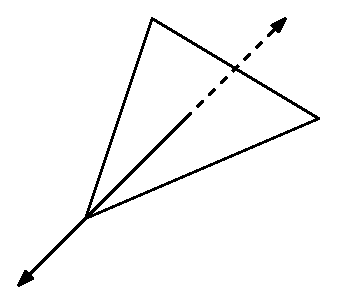
\includegraphics[scale=0.5]{src/geo/gfx/fig/pasch.eps}
\caption{\label{fig:pasch}Pasch's Axiom}
\end{center}
\end{figure}

\begin{lem}
Let \(\ell\) be a line and \(C \in \ell\) a point in an ordered geometry.
Suppose \(A\) and \(B\) are points not on \(\ell\) such that \(\BETWEEN{A}{B}{C}\).
Then \(A\) and \(B\) are on the same side of \(\ell\).
\end{lem}

\begin{proof}
Suppose otherwise that \(A\) and \(B\) are on opposite sides of \(\ell\).
By the Plane Separation property, and because \(A\) and \(B\) are not on \(\ell\), the segment \(\SEGMENT{A}{B}\) cuts \(\ell\) at a unique point \(D\).
That is, \(D \in \ell\) and \(\BETWEEN{A}{D}{B}\).
But note that \(C, D \in \ell\), so \(\LINE{C}{D} = \ell\), and also \(C, D \in \LINE{A}{B}\), so that \(\LINE{C}{D} = \LINE{A}{B}\).
But then \(\LINE{A}{B} = \ell\), a contradiction.
Thus \(A\) and \(B\) must be on the same side of \(\ell\).
\end{proof}

%---------%
\Exercises%
%---------%
